% !TeX root = ../paper.tex
\begin{figure}[t]
  \centering
  \setlength{\parskip}{0pt}
  % One body-line gap before the caption; retain the standard float-to-text gap.
  \setlength{\abovecaptionskip}{\baselineskip}
  \setlength{\belowcaptionskip}{0pt}
  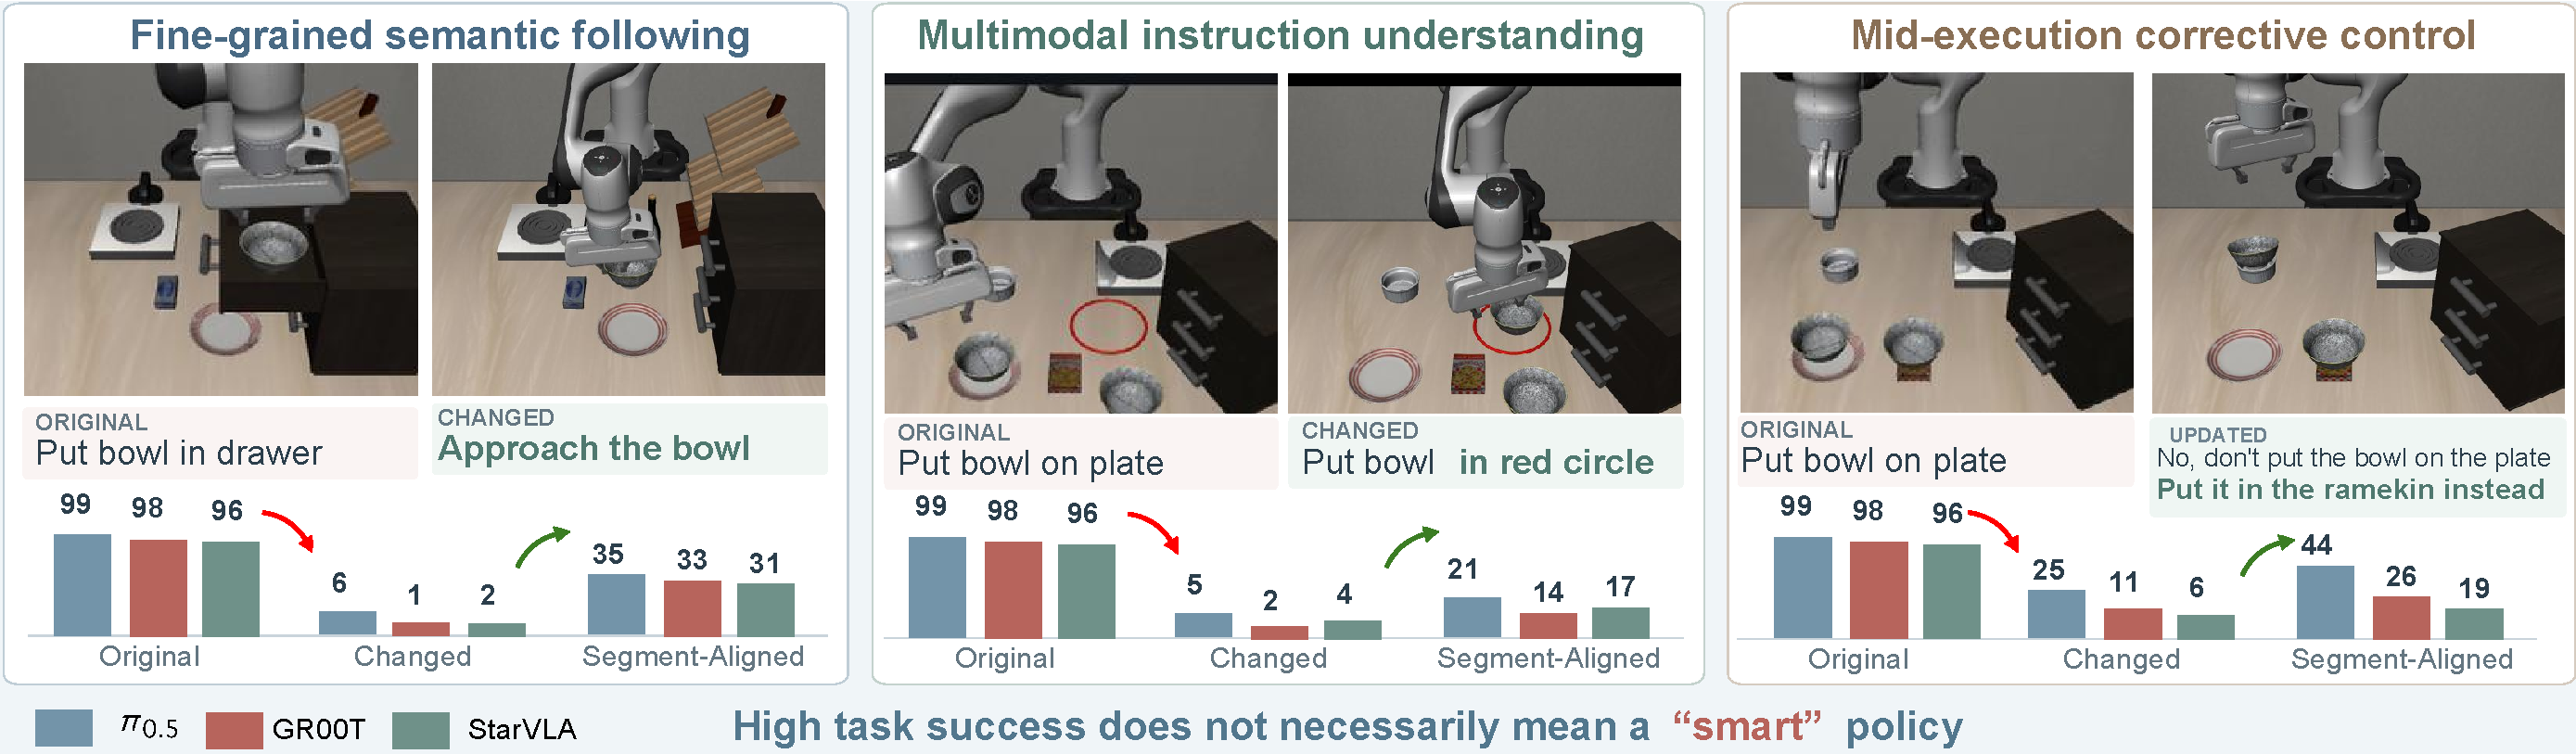
\includegraphics[width=\textwidth,pagebox=cropbox]{figures/1--figure1_editable.pdf}\par\nointerlineskip
  \caption{Instruction-following diagnosis across fine-grained semantic following, multimodal
  instruction understanding, and mid-execution corrective control. Bars compare success rates
  (\%) under original instructions, changed or updated instructions, and segment-aligned
  supervision for $\pi_{0.5}$, GR00T, and StarVLA. High original-task success can coexist with
  poor instruction following, while segment-aligned supervision improves performance under
  the changed requirements.}
  \label{fig:overview}
\end{figure}
